\chapter{Smart Contract Security}

\section{Introduzione}

Come per altri programmi, un Smart Contract eseguirà esattamente ciò che è scritto,
che non sempre è ciò che il programmatore intendeva. Tutti i contratti smart sono
pubblici e qualsiasi utente può interagire con essi semplicemente creando una
transazione.
Una volta che la transazione viene mandata sulla blockchain, significa che fa parte
di un blocco e non può essere più annullata.
I dati della transazione sono inalterabili anche perché
sono distribuiti.
Gli Smart Contract possono gestire denaro, ma una volta perso è praticamente
impossibile recuperarlo.
Il codice dello Smart Contract è spietato. Ogni bug può portare a perdite
monetarie.
La complessità è nemica della sicurezza. Più semplice è il codice,
minori sono le possibilità
che si verifichi un bug o un effetto imprevisto. Quando ci si impegna per la
prima volta nella
programmazione di uno Smart Contract, gli sviluppatori sono spesso tentati di
provare a scrivere codice molto codice ed articolato.
Invece, si dovrebbe trovare il modo per fare meno, con meno linee di
codice, meno complessità e meno "features".
Se esiste già una libreria o un contratto che fa gran parte del necessario,
riutilizzatela.
All'interno del codice, seguite il principio \textit{DRY}: Don't Repeat Yourself.
Attenzione alla sindrome del "Not Invented Here", dove si è tentati di
"migliorare" una caratteristica o un componente costruendola da zero.
Non si dovrebbe trattare la programmazione a Smart Contract allo stesso modo della
programmazione generale. Piuttosto, si dovrebbero applicare rigorose metodologie di
ingegneria e di sviluppo software.
Una volta "lanciato" il vostro codice, c'è poco da fare per risolvere eventuali
problemi.
Il vostro codice deve essere chiaro e facile da comprendere.
Più è facile da leggere, più è
facile da controllare.
I contratti intelligenti sono pubblici, poiché tutti possono leggere il bytecode
e chiunque può
invertirlo e modificarlo. Pertanto, è utile sviluppare il proprio lavoro in
pubblico, utilizzando
metodologie collaborative e open source, per attingere alla saggezza collettiva.
Dato che l'ambiente di esecuzione è pubblico, prima di poter essere lanciato,
il codice deve essere
testato in maniera approfondita.
Vanno soprattutto analizzati i possibili input maligni e i loro effetti.

\section{IF e REQUIRE}

\begin{lstlisting}
    if(_newDelegate != delegateContract){
        // Do something
    }

    require(_newDelegate != delegateContract){
        // Do something
    }
\end{lstlisting}

\paragraph{IF.}
È solo un'esecuzione condizionale del blocco \verb|// Do something|.
Quindi, se questa condizione non
è soddisfatta, \verb|// Do something| viene saltato.

\paragraph{REQURIE.}
Controlla sempre una condizione ma,
se non si avvera, la transazione viene abortita e
ripristinata. Viene rimborsato anche il gas.
\ \\
\paragraph{Esempio.}\

\begin{lstlisting}
uint256 input;
address sender;
function some_state_changing_fn(uint256 _input) public 
  returns (bool success) {
     sender = msg.sender;
     require(_input >= 100);
     input = _input;
     success = true;
}
\end{lstlisting}

\verb|sender| è l'indirizzo di chi chiama la transazione e spedisce denaro.
Il corpo della funzione salva in \verb|sender| l'indirizzo \verb|msg.sender|.
\verb|msg| è il messaggio che viene
mandato al contratto. \verb|require| richiede che l'input passato sia $ > 100$.
Se il valore passato \verb|_input| nella transazione è $ > 100$,
allora si aggiorna la variabile \verb|input|.
Altrimenti fallisce. Aggiornando \verb|input| si aggiorna lo stato del contratto.

\section{DAO Attack}

\subsection{Reentrancy}

Una delle caratteristiche degli Smart Contract di Ethereum è la loro capacità di
richiamare e utilizzare il codice di altri contratti esterni. I contratti
gestiscono l'ether e spesso lo inviano a
vari indirizzi di utenti esterni. Queste operazioni richiedono ai contratti di
inviare appunto call esterne.
Queste chiamate possono essere dirottate dagli aggressori, i quali potrebbero
costringere i contratti ad eseguire ulteriori codici
(attraverso una funzione di fallback). Attacchi di questo
tipo sono stati utilizzati nel famigerato hack DAO.
Il 17 giugno 2016 il DAO è stato violato e $3,6$ milioni di ether ($658.002.709$ euro)
sono stati rubati con quello che viene considerato i primo attacco di reentrancy.

\subsection{Attacco}

In Solidity esistono 3 funzioni per il trasferimento di ether: \verb|someAddress.send()|,
\verb|someAddress.transfer()| e \verb|someAddress.call.value()|.
Da notare che \verb|x.transfer(y)| è equivalente a \verb|require(x.send(y))|.
\verb|send| e \verb|transfer| sono sicure contro il \textit{reentrancy} perché
hanno associato un certo limite di operazioni possibili.
Infatti, se la funzione eseguita consuma più del limite imposto da \verb|send| e \verb|transfer|,
si interrompe l'esecuzione.
Al contratto chiamato viene assegnato solo uno valore di $2300$
gas, sufficiente solo per registrare un certo evento.
Il gas in generale permette di evitare DoS. Dovendo gestire pagamenti,
si fa in modo che le chiamate a funzioni dei contratti siano limitate, è un modo
per proteggere la blockchain.
Se la transazione fallisce, viene effettuata un'operazione di ripristino (revert)
automatico, cioè si ritorna allo stato originale.\\
A differenza delle due precedenti, \verb|someAddress.call.value(y)()| non ha questo
tipo di protezione, invocandola verrà inviato
l'ether specificato e farà scattare
l'esecuzione di una specifica parte di codice del contratto chiamante
(funzione di \textit{fallback}).
Il codice eseguito viene fornito con tutto il gas
disponibile per l'esecuzione, rendendo
questo tipo di trasferimento di valori unsafe contro il reentrancy.
Non ci sono quindi limiti, si può andare anche oltre $2300$ gas.

\paragraph{ESEMPIO.}\ \\
\verb|contract.sol|\\
Di seguito il codice di uno Smart Contract simile a quello del DAO Attack.

\begin{figure}[H]
      \centering
      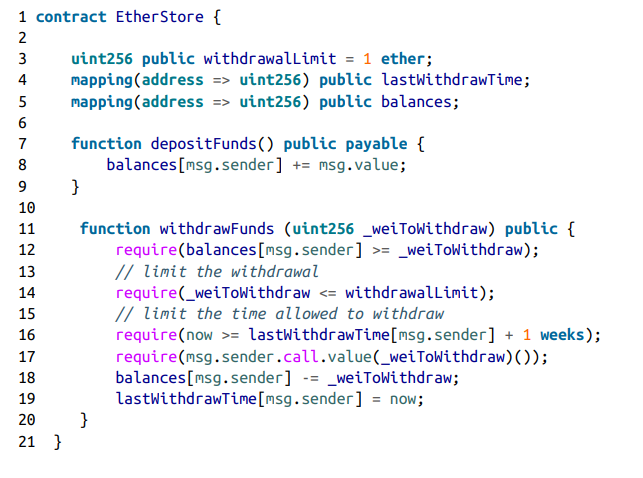
\includegraphics[width=10cm, keepaspectratio]{capitoli/ethereum/imgs/dao_buono.png}
      \caption{Codice del contratto contract.sol}
\end{figure}

Abbiamo due funzioni. La prima, \verb|depositFunds|, permette di depositare
appunto i fondi.
La funzione ha l'attributo \verb|payable|: fornisce un meccanismo per
raccogliere/ricevere fondi in ether per il contratto.
Nella funzione viene aggiornato il bilancio del mittente con \verb|msg.value|.
\verb|balance| è un array dei depositari, mentre \verb|msg.value| indica la
quantità di ether che viene trasferita.
La funzione \verb|withdrawFunds|, invece, serve per ritirare.
Prende come parametro una certa quantità di denaro.
Ha una serie di \verb|require|:

\begin{enumerate}
      \item Richiede che il bilancio depositato sia maggiore di quello ritirato;
      \item Il bilancio ritirato deve essere minore di un certo limite
            (stabilito arbitrariamente);
      \item Verifica che sia passato del tempo dall'ultima richiesta di ritiro di
            denaro;
      \item Trasferisce gli wei attraverso la funzione \verb|msg.sender.call.value|
            che non ha limiti sul gas;
\end{enumerate}

Alla fine si aggiorna il bilancio di \verb|msg.sender| e lo stato interno,
compreso il momento in
cui è avvenuta la transazione (\verb|now|).\ \\

\verb|attack.sol|\ \\
Di seguito il codice del contratto scritto per attaccare il precedente.

\begin{figure}[H]
      \centering
      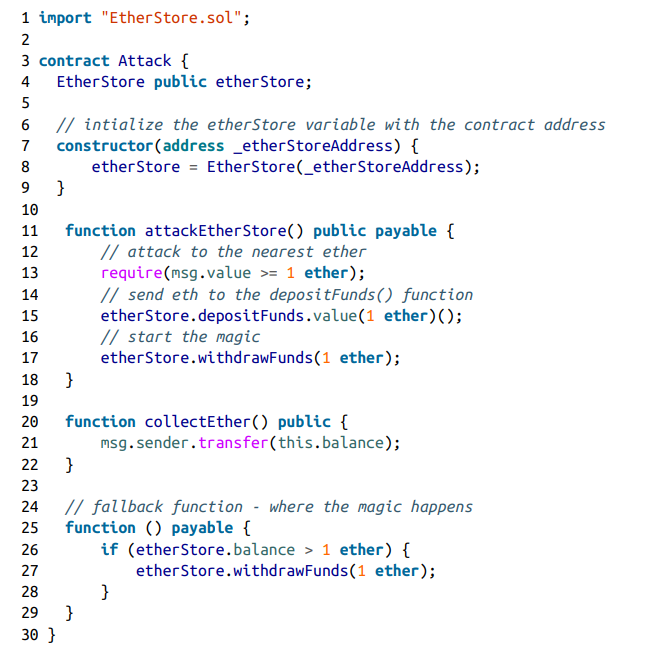
\includegraphics[width=10cm, keepaspectratio]{capitoli/ethereum/imgs/dao_cattivo.png}
      \caption{Codice del contratto attack.sol}
\end{figure}

Il costruttore viene inizializzato con l'indirizzo del contratto che si vuole
attaccare: viene memorizzato nella variabile \verb|etherStore| e quindi
chiaramente anche nella blockchain.
Il trasferimento di denaro avviene tramite la funzione \verb|collectEther|.
Chiamo il contratto e
quindi anche questa. Trasferisco una certa quantità di ether $ >=1$
(per come stabilisce il \verb|require|). L'Ether viene inviato a \verb|etherStore|,
cioè il contratto che si vuole attaccare.
Sul contratto di attacco c'è depositato 1 ether.
Gli chiedo di aggiungerne 1 altro sul precedente chiamando \verb|withdrawFunds|.
Avviene quindi il versamento e poi l'ulteriore
richiesta.
Se non viene specificata una funzione in particolare,
viene chiamata di default la fallback.
Le funzioni di fallback in Solidity vengono eseguite quando un identificatore di
funzione non corrisponde a nessuna delle funzioni disponibili in un contratto
oppure se non sono stati
forniti dati. Sono senza nome, non possono accettare argomenti, non possono
restituire nulla e ci può essere solo una funzione di fallback.
Sono una sorta di valvola di sicurezza.
In breve, il contratto di attacco ha versato 1 ether ma allo stesso tempo sta
effettuando più volte di seguito la richiesta di ritirarne 1.
Il problema è che l'aggiornamento del \verb|balance| viene
effettuato soltanto dopo la spedizione del denaro. Per cui (per esempio) invece
di chiederne 1 ne chiedo e ne ricevo 2.
Ritiriamo di più di quanto effettivamente richiesto.
La funzione in realtà sta aspettando una risposta e il conseguente aggiornamento, ma
vengono solo sottratti ulteriori ether. L'attacco va a buon fine in quanto il controllo sul
bilancio viene effettuato soltanto alla fine.

\paragraph{RICAPITOLANDO.}\ \\
Per sfruttare la vulnerabilità dovuta dalla funzione \verb|someAddress.call.value()|
procedo nel seguente modo:

\begin{enumerate}
      \item Effettuo una transazione al contratto malvagio (\verb|attack.sol|) di almeno
            1 ether (\verb|require| alla riga 13 di \verb|attack.sol|)
      \item 1 ether viene depositato sul contratto bersaglio (\verb|contract.sol|) invocando
            la funzione \verb|depositFunds| (riga 15 di \verb|attack.sol|)
      \item Chiedo al contratto bersaglio di ritirare i fondi che ho depositato
            (riga 17 di \verb|attack.sol|). È proprio qui che inizia la \textit{magia}.
      \item  Viene eseguita la funzione \verb|withdrawFunds| (riga 11 di \verb|contract.sol|).
            Tutti i \verb|require| vengono superati e viene inviato il denaro al contratto attaccante
            (riga 17 di \verb|contract.sol|).
      \item Questo invio non fa continuare l'esecuzione della funzione \verb|withdrawFunds|
            andando a modificare il bilancio, ma triggera l'esecuzione della funzione
            di fallback del contratto attaccante.
      \item  Viene eseguita la funzione di fallback del contratto attaccante
            (riga 25 di \verb|attack.sol|) che continuerà a richiedere soldi
            (e li otterrà) fin
            quando il bilancio del contratto bersaglio non finirà, impedendo
            per tutto il tempo che la riga 18 di \verb|contract.sol| venga eseguita.
\end{enumerate}

\subsection{Mitigation}

Per cercare di arginare questa falla si usa una combinazione di più accorgimenti:

\begin{enumerate}
      \item Usiamo una mutex, ovvero una variabile booleana subito all'inizio
            del ritiro. Altrimenti chi ha chiamato continuerebbe a farlo senza problema.
            Se la variabile booleana è
            settata nel modo corretto (all'inizio è a false), si bloccano gli accessi.
            Non si entra nel
            contratto se la mutex non è stata sbloccata.
      \item Aggiorno il bilancio prima di trasferire i soldi al chiamante.
            Prima trasferivo i soldi e
            poi aggiornavo il bilancio, ora il contrario.
            Cio è accompagnato dallo sblocco del
            mutex.
      \item Viene usata la \verb|transfer| con il suo limite di gas che causa
            quindi un limite per l'
            esecuzione.
\end{enumerate}

\section{Arithmetic underflow/overflow}

\begin{figure}[H]
      \centering
      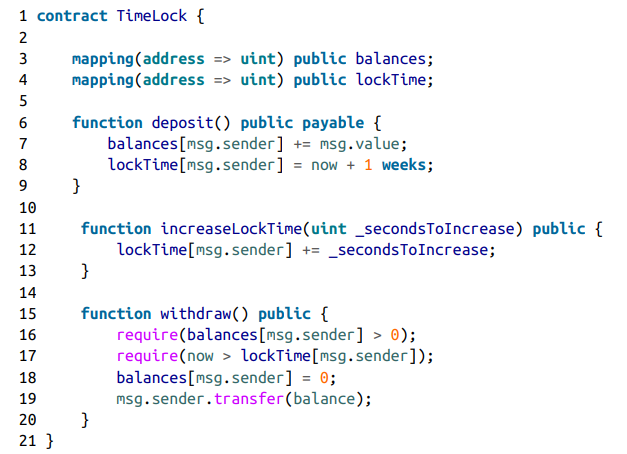
\includegraphics[width=10cm, keepaspectratio]{capitoli/ethereum/imgs/aritmetic.png}
      \caption{Esempio di codice dove vulnerabile ad Arithmetic underflow/overflow.}
\end{figure}

La keyword \verb|mapping| fungono da tabelle di hash che consistono in coppia
\verb|chiave-valore|. In questo caso abbiamo 2 mapping: \verb|balances| e \verb|lockTime|,
il primo associa ogni indirizzo ethereum di chi chiama questo contratto ad un numero
che rappresenta il saldo di quell'indirizzo; il secondo associa ad ogni indirizzo
un numero che rappresenta il lock-time (quanto deve passare da un ritiro all'altro).
La funzione \verb|deposit| incrementa il saldo dell'indirizzo chiamante (\verb|msg.sender|)
di quanto ha versato (\verb|msg.value|) (riga 7). Viene anche impostato il lockTime
dello specifico indirizzo ad 1 settimana (riga 8): tra 1 settimana sarà possibile ritirare i fondi.
La funzione \verb|increaseLockTime| permette di allungare il \verb|lockTime|, specificando
il numero di secondi.
La funzione \verb|withdraw|, dopo aver controllato se abbiamo abbastanza denaro
(riga 16) e che sia trascorso il \verb|lockTime| (riga 17), viene azzerato
il bilancio (riga 18)
e trasferiti, in modo sicuro, tutti i soldi all'indirizzo del chiamante (riga 19).
Il problema però è in \verb|increaseLockTime| (riga 11).
La variabile richiesta è un uint: se sommassi un
numero sufficientemente alto di secondi, farei il giro completo dei uint e
ripartirei da 0.
Per cui avrei dei numeri molto piccoli.
Questo potrebbe rappresentare un tentativo di attacco.
L'aggiunta di numeri più grandi dell'intervallo del tipo di dati causa un overflow.
Da notare che la stessa cosa vale per l'underflow: sottrarre a $0$ una certa
quantità porterà ad avere il massimo numero rappresentabile in uint.
Così facendo posso andare a resettare il limite di tempo imposto da \verb|lockTime|.

\subsection{Mitigation}

La tecnica normalmente utilizzata per proteggersi dalle vulnerabilità di
under/overflow è
quella di utilizzare o costruire librerie matematiche che sostituiscono gli
operatori matematici
standard di addizione, sottrazione e moltiplicazione.
Per esempio, OpenZeppelin è una
libreria per lo sviluppo sicuro di un Smart Contract.

\section{Unexpected Ether}

Ci sono dei casi in cui è possibile mandare ether ad un contratto senza che ci
sia una funzione a riceverlo.
In genere, quando l'ether viene inviato ad un contratto, deve eseguire la
funzione di fallback o un'altra funzione definita nel contratto.
Ci sono due eccezioni a questo, in cui l'ether può
esistere in un contratto senza aver eseguito alcun codice.
I contratti che basano l'esecuzione
del codice su tutto l'ether che gli viene inviato possono essere vulnerabili ad
attacchi in cui
viene appunto inviato con la forza.
Un contratto può avere proprio una funzione senza nome,
che può non avere argomenti, né
restituire nulla. Le funzioni di fallback vengono eseguite se un contratto viene
chiamato e
nessun'altra funzione corrisponde all'identificatore di funzione specificato
o se non vengono forniti dati.
Una tecnica di programmazione difensiva comune, utile per far rispettare le
corrette transizioni di stato o per convalidare le operazioni, è
l'\textit{invariant checking}. Questa tecnica
consiste nel definire un insieme di invarianti
(metriche o parametri che non dovrebbero
cambiare) e nel verificare che questi rimangano invariati dopo una singola (o molte)
operazioni.
Come accennato in precedenza, ci sono due modi in cui l'ether può (forzatamente)
essere
inviato ad un contratto senza utilizzare una funzione \verb|payable| o eseguire
codice sul contratto:

\begin{enumerate}
      \item \textbf{Self-destruct}: una funzione che permette di rimuovere il
            contratto dalla blockchain.
            Può essere chiamata solo da chi ha creato il contratto;
      \item \textbf{Pre-sent ether}: mandare ether preventivamente.
\end{enumerate}

\paragraph{Self-destruct.}

Rimuove tutti i bytecode dall'indirizzo del contratto e sposta tutto l'ether
lì memorizzato all'indirizzo specificato dal parametro. Se anche questo
indirizzo specificato è un contratto,
non viene chiamata nessuna funzione, neanche la fallback. Pertanto, la funzione di
self-destruct può essere utilizzata per l'invio forzato di ether a qualsiasi
contratto,
indipendentemente dal suo codice e anche ai contratti senza funzioni payable.
Ciò significa che ogni attaccante può creare un contratto e con una funzione di
\verb|self-destruct|,
inviare ether ad esso: non si fa altro che chiamare \verb|selfdestruct(target)|
e forzare
l'invio dell'ether ad un certo contratto target.

\paragraph{Pre-sent ether.}

Un altro modo è quello di pre-caricare l'indirizzo del contratto con l'ether da
inviare. Gli
indirizzi del contratto sono creati in modo deterministico: l'indirizzo è
calcolato dall'hash \verb|Keccak-256| a partire dall'indirizzo che crea il
contratto e dalla \verb|nonce| (è un
contatore che viene incrementato solo quando quel contratto ne crea un altro).
Ciò significa
che chiunque può calcolare l'indirizzo di un contratto prima che venga creato e
inviargli ether.

\section{Default Visibilities}

Le funzioni in Solidity hanno specificatori di visibilità che indicano come
possono essere chiamate. La visibilità determina se una funzione può essere
chiamata esternamente dagli utenti o da altri contratti derivati, solo internamente
oppure solo esternamente.
Ci sono quattro specificatori di visibilità: \textbf{external}, \textbf{public},
\textbf{internal}, \textbf{private}.
Le funzioni di default sono \verb|public| e permettono agli utenti di chiamarle
esternamente da chiunque nel mondo, una volta che il contratto è sulla blockchain.
Vedremo ora come l'uso scorretto degli specificatori di visibilità può portare
ad alcune vulnerabilità negli Smart Contract.
Il problema si pone quando gli sviluppatori omettono erroneamente gli
specificatori di
visibilità sulle funzioni che dovrebbero essere \verb|private|.

\begin{figure}[H]
      \centering
      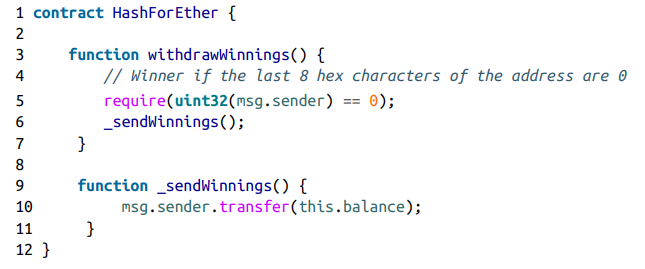
\includegraphics[width=12cm, keepaspectratio]{capitoli/ethereum/imgs/visibility.png}
      \caption{Codice vulnerabile a questo tipo di attacco.}
\end{figure}

Esaminiamo il codice del contratto qui sopra.
La funzione \verb|withdrawWinnings| stabilisce chi
vince: se le ultime 8 cifre dell'hash
del nostro indirizzo sono pari a $0$
allora siamo noi i vincitori.
\verb|_sendWinnings| si occupa di
mandare la vincita.
Dato che però il contratto è
pubblico, tutti lo possono vedere;
ciò significa che tutti possono chiamare le sue funzioni, compresa
\verb|_sendWinnings|.
Invece di giocare, chiamo direttamente la funzione per la consegna della vincita e
ritiro tutto
il denaro del bilancio del contratto, anche se la logica porterebbe diversamente.
\verb|_sendWinnings| doveva quindi avere visibilità \verb|private|.

\section{Entropy Illusion}

Tutte le transazioni sulla blockchain dell'Ethereum sono operazioni di
transizione a stato deterministico. Ciò significa che ogni transazione
modifica lo stato globale del sistema
Ethereum in modo calcolabile, senza alcuna incertezza e soprattutto randomizzazione.
Tutto ciò che passa sulla blockchain deve essere validato dall'intera rete di
miners, per cui non è
possibile che ognuno di loro ottenga valori (randomici) differenti.
Non può esserci entropia o
casualità in Ethereum.
Il raggiungimento dell'entropia decentralizzata (casualità) è un problema ben noto
per il
quale sono state proposte molte soluzioni: vedremo infatti il \verb|RandDAO|.
Molti dei contratti di Ethereum sono basati sul gioco d'azzardo, il quale
fondamentalmente
richiede un po' di casualità cioè qualcosa su cui scommettere;
ciò rende la costruzione di un
sistema di gioco d'azzardo a catena (ma su base deterministica) piuttosto difficile.
Una pratica comune è quella di utilizzare le future variabili di blocco,
cioè le variabili che
contengono informazioni sul blocco delle transazioni i cui valori non sono ancora
noti (hash, timestamp, numeri di blocco o gas limit).
Questi valori però sono controllati dal miner che
estrae il blocco e pertanto non sono del tutto casuali.

\paragraph{Esempio.}\ \\

Si consideri uno Smart Contract di roulette che restituisce un numero nero se il
blocco successivo termina con un numero pari.
Un miner (o miner pool) potrebbe scommettere 1 milione di dollari sul nero.
Se il blocco
successivo viene risolto e si trova l'hash finito in un numero dispari,
il miner potrebbe
tranquillamente non pubblicare il blocco ed estrarne un altro,
fino a quando non trova una
soluzione con l'hash del blocco come numero pari (supponendo comunque che la
ricompensa del blocco e le tasse siano meno di 1 milione di dollari).

\subsection{Mitigation}

Per i motivi elencati prima, le block variables non dovrebbero essere usate per
generare entropia, in
quanto possono essere manipolate dai miner.
La sorgente dell'entropia (casualità) dovrebbe essere esterna alla blockchain.
Ciò può
essere ottenuto cambiando il modello di trust in un gruppo di partecipanti,
come avviene in
\verb|RandDAO|. Viene creata infatti una sorta di “terza parte” che si fa garante
della creazione di
variabili casuali ma ciò allo stesso tempo avviene in modo distribuito.
Le regole quindi sono riassunte in un contratto: abbiamo pegno, invio di una parte
del seed,
generazione di un numero aleatorio, restituzione del pegno più parte delle tasse.
Questo è un DAO: Organizzazione Anonima Decentrata.

\section{Manipolazione dei Time Blockstamp}

I minatori hanno la possibilità di regolare leggermente i timestamp,
il che può rivelarsi
pericoloso se essi venissero utilizzati in modo scorretto.

\paragraph{Esempio.}\ \\

\begin{figure}[H]
      \centering
      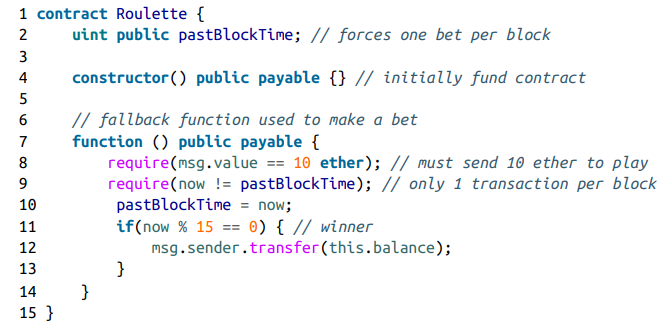
\includegraphics[width=12cm, keepaspectratio]{capitoli/ethereum/imgs/timestamp.png}
      \caption{Sezione di codice vulnerabile alla Timestamp Manipulation.}
\end{figure}

Prendiamo in considerazione in precedente codice di un contratto che simula
una roulette.
Chiunque può puntare 10 ether (riga8 ).
Il secondo \verb|require| (riga 9) controlla che ci sia una
sola transazione nel nuovo blocco;
poi questa verrà aggiornata subito,
per indicare il fatto che qualcuno ha già giocato.
Supponiamo che qualcuno ha
esattamente puntato in questo
momento, ovvero quando si
verifica la condizione $now \%15 ==  0$ (riga 11); allora lui sarà
il vincitore e con la \verb|transfer| (riga 12)
riceverà tutto il denaro che è stato versato dagli altri giocatori nelle
transazioni precedenti.
In realtà, \verb|now| è leggermente modificabile.
Di conseguenza, potrebbe accadere che il
miner aggiusti il tempo in cui punta e in cui mina il blocco,
in modo che la condizione si
verifichi (parliamo sempre di una modifica molto piccola).

\section{Delegate Call}

Gli opcode \verb|CALL| e \verb|DELEGATECALL| permettono lo sviluppo modulare
del codice di un contratto di Ethereum.
Tuttavia con \verb|DELEGATECALL| l'esecuzione del codice specificato
nell'indirizzo viene eseguita utilizzando il contesto del contratto chiamante,
cosa che non si verifica con \verb|CALL|.
Questo può causare delle vulnerabilità che vedremo ora con un esempio.

\subsection{Attacco}

\begin{figure}[H]
      \centering
      \begin{subfigure}[b]{.5\textwidth}
            \centering
            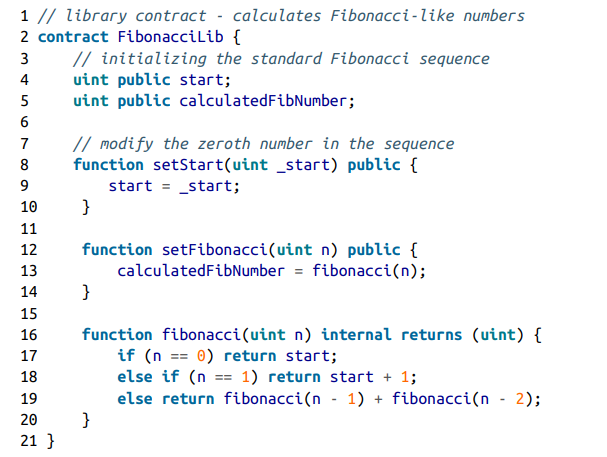
\includegraphics[width=\linewidth, keepaspectratio]{capitoli/ethereum/imgs/delegate_lib.png}
            \caption{FibonacciLib.sol.}
      \end{subfigure}%
      \begin{subfigure}[b]{.5\textwidth}
            \centering
            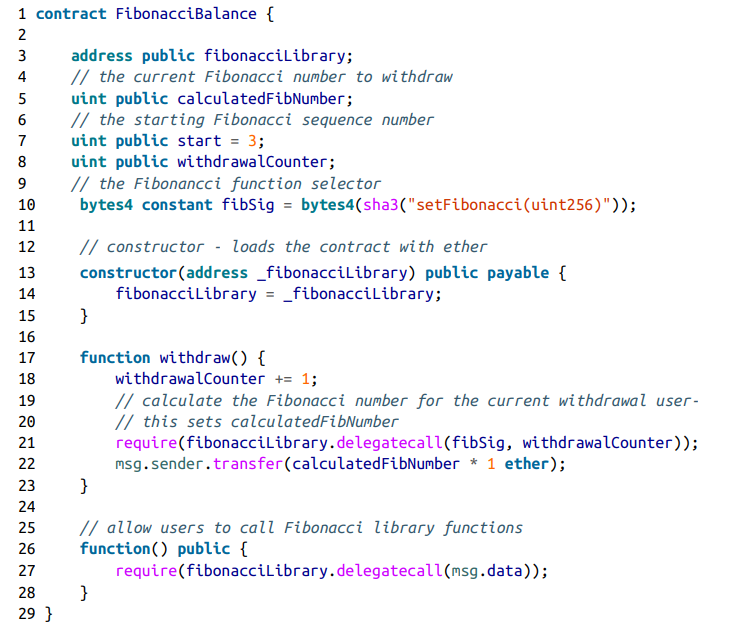
\includegraphics[width=\linewidth, keepaspectratio]{capitoli/ethereum/imgs/delegate_contratto.png}
            \caption{FibonacciContratto.sol.}
      \end{subfigure}
\end{figure}

Prendiamo come esempio una libreria che può generare l'n-esimo numero di fibonacci
e che ha una funzione \verb|setStart| che ci permette di cambiare il numero
iniziale della sequenza (figura a).
Ora creiamo un contratto (figura b) che andrà ad utilizzare questa libreria e
permetterà il prelievo di ether in base al numero della posizione di fibonacci
che corrisponde all'ordine della nostra richiesta.
Questo contratto ha una fallback function (riga 26 di b)
che ci permette di chiamare qualsiasi funzione presente nella libreria.
Se per chiamare le funzioni della libreria utilizziamo \verb|delegatecall|,
a causa del contesto utilizzato possono insorgere problemi di sicurezza.\\
Le variabili nei contratti vengono salvate in una lista (\verb|slot|)
che parte dalla posizione $0$ ed è relativa al contesto del contratto,
dunque se nella libreria abbiamo la variabile nella posizione $0$ (\verb|slot[0]|)
che corrisponde a \verb|start| (riga 4 di a) e chiamiamo la funzione
\verb|setStart| con \verb|delegatecall|, non utilizzeremo la variabile in
posizione $0$ nella libreria me quella del contratto chiamante,
che nel nostro caso corrisponde all'indirizzo del contratto (libreria).
Questo permette ad un utente malevolo di
cambiare l'indirizzo della libreria a piacimento, dirottando l'esecuzione
del codice in un contratto malevolo che può anche essere in grado di svuotare
tutto il conto del contratto vittima.

\subsection{Mitigation}

Per evitare questa vulnerabilità, Solidity mette a disposizione la keyword
\verb|library| per implementare contratti \textit{stateless}.
Questo risolve i problemi di complessità, gestione dello stato della libreria ed
impedisce la modifica dello stato come visto nell'esempio in precedenza.
Se invece dobbiamo per forza utilizzare librerie state-full vanno controllati
con estrema attenzione i possibili cambiamenti di stato indesiderati e side effects.
Come regola generale vanno sempre utilizzate librerie stateless quando possibile.

\section{Unchecked Call Return Values}

In Solidity ci sono delle funzioni che permettono di mandare ether ad account
esterni. Comunemente viene utilizzata la funzione \verb|transfer|, ma ci sono
altri metodi per farlo. Le funzioni \verb|call| e \verb|send| sono metodi
alternativi che però richiedono particolari attenzioni, poiché entrambe
ritornano valori booleani: \verb|true| se la transazione ha avuto successo e
\verb|false| altrimenti. Un programmatore inesperto potrebbe aspettarsi che se
la transazione fallisce, verrebbe effettuato in automatico il revert.
Tuttavia questo avviene solo se viene esplicitamente controllato il valore di
ritorno di \verb|call| e \verb|send|, altrimenti l'esecuzione prosegue senza errori.

\subsection{Attacco}

\begin{figure}[H]
      \centering
      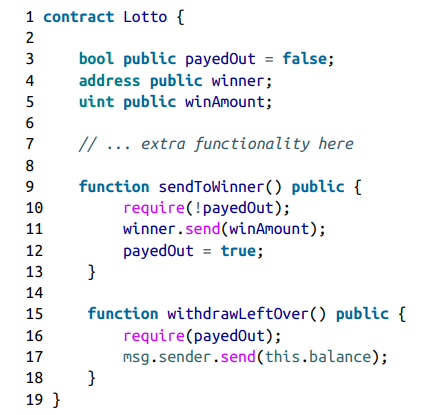
\includegraphics[width=6cm, keepaspectratio]{capitoli/ethereum/imgs/unchecked_call.png}
      \caption{Codice soggetto a questo tipo di vulnerabilità.}
\end{figure}

Prendendo in considerazione il precedente contratto, in cui andiamo a simulare
la Lotteria: viene scelto un utente vincitore che può ritirare la somma vincente,
mentre viene lasciata a disposizione una piccola quantità di denaro ritirabile
dagli altri utenti solo dopo la riscossione della vincita.
La vulnerabilità è presenta alla riga 11, dove la funzione \verb|send| viene
invocata senza controllare il suo valore di ritorno. Se fallisce l'invio della
vincita, per colpa del numero insufficiente di gas o per via dell'account del
vincitore, tutta la vincita viene lasciata a disposizione della funzione
\verb|withdrawLefOver| e chiunque potrà ritirare l'intera vincita.
Questo perché la riga 11 non effettua in automatico il revert e continua
con l'esecuzione della riga 12.

\subsection{Mitigation}

Per risolvere questo problema va utilizzata la funzione \verb|transfer|
quando possibile oppure una soluzione più robusta è quella di adottare dei
\textit{withdraw pattern} in cui ogni utente chiama una funzione di prelievo
isolata che gestisce tutte le possibili situazioni.

\section{Race Conditions/Front Running}

Quando un contratto viene incluso in un blocco da un miner,
questa inclusione avviene dando precedenza a transazioni che hanno determinati
parametri come il \verb|gasPrice| più alto.
Questo è un potenziale vettore d'attacco in quanto un attaccante può osservare
la pool delle transazioni, cercandone alcune che hanno soluzioni a problemi con
vincite in denaro. L'attaccante può quindi mandare la stessa soluzione dell'utente
che l'ha risolta con un \verb|gasPrice| maggiore per incrementare la probabilità
che la sua transazione venga validata prima, così facendo otterrà la vincita
che spettava all'altro utente.

\subsection{Mitigation}

Ci sono due metodi principali per difendersi da questi attacchi,
il primo è quello di imporre un \textit{upper bound} al \verb|gasPrice|
per impedire che gli utenti possano alzarlo sempre di più;
il secondo è quello di utilizzare uno schema \textit{commit-reveal},
tale schema impone che vengano inclusi dati nascosti nella transazione
(di solito un hash) che verranno rivelati nella fase di reveal,
impedendo così queste race condition o front running.

\section{DoS}

Gli attacchi di questo tipo consistono nel rendere un contratto temporaneamente
o permanentemente inoperabile.
Noi ci concentreremo su attacchi meno ovvi e conosciuti.

\subsection{Attacchi}

\begin{itemize}
      \item \textit{Looping through externally manipulated mappings or arrays}:
            in questo tipo di attacchi, l'attaccante può creare molti account aumentando
            la dimensione dell'array in maniera tale che la richiesta di gas superi il
            limite disponibile, rendendo l'esecuzione del contratto impossibile.
            \begin{figure}[H]
                  \centering
                  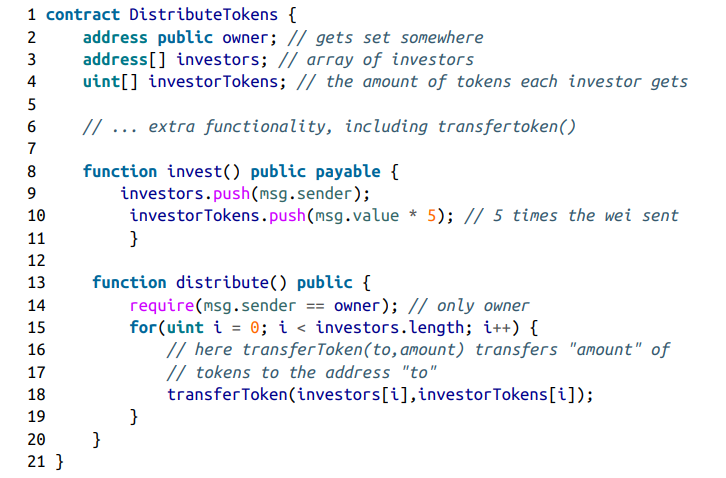
\includegraphics[width=10cm, keepaspectratio]{capitoli/ethereum/imgs/dos_looping.png}
            \end{figure}
      \item \textit{Owner Operations}:
            se una funzione richiede permessi speciali per essere eseguita,
            e l'utente che li ha perde la sua chiave privata,
            allora tutta la funzione diventerà inoperabile
      \item \textit{Progressing state based on external calls}:
            alcuni contratti vengono a volte scritti in maniera tale da richiedere
            interventi esterni come invio di denaro o operazioni varie per poter
            proseguire. Se questi interventi esterni vengono impediti per qualche motivo,
            questo risulterà essere un attacco DoS.
\end{itemize}

\subsection{Mitigation}

Per evitare il primo tipo di attacco,
basta evitare che i contratti iterino all'interno di strutture dati manipolabili
da utenti esterni. È raccomandato l'utilizzo di un \textit{withdraw pattern}.\\

Nel secondo caso può essere utile creare un \textit{failsafe} utilizzabile nel
caso in cui un utente owner diventi incapacitato.
È anche possibile rendere l'owner un contratto \textit{multisig}.
Un'altra soluzione è quella di utilizzare un \verb|timelock| grazie al quale il
contratto terminerà dopo un periodo di tempo specificato.
Queste tecniche possono essere anche utilizzate nel terzo esempio.